% !TEX root =  ../main.tex
\section{SingleCapacity}

\subsection{Definition}

\subsubsection{Signature} \cstr{singleCapacity(s:set<server>, nb:number, r:string)}

\begin{itemize}
\item \cstr{s}: a non-empty set of servers for a meaningful constraint. Servers not in the \st{Online}
state are ignored.
\item \cstr{r} : a resource identifier such as \cstr{mem}, \cstr{ucpu}, \cstr{pcpu} or \cstr{vm} to identify the physical memory,
the computational capacity, the physical CPUs or the number of hosted VMs, respectively.
\item \cstr{nb}: a positive amount of resources.
\end{itemize}


The \cstr{singleCapacity} constraint restricts to a maximum of \cstr{nb}, the amount
of a specific resource of type \cstr{r} that can be used on each of the online servers
in \cstr{s} to run VMs.

\classification{singleCapacity}{datacenter administrator}{VM placement,Resource allocation}{Resource management,VM-to-server placement}

\subsubsection{Usage}

The \cstr{singleCapacity} constraint is used by a datacenter administrator to indicate to the VM manager,
the practical amount of resources on each server, that will be available to the VMs.
As an example, a server having 4~GB of RAM running a Xen hypervisor~\cite{xen-sosp03} cannot offer this
amount of memory to the VMs as the \emph{Domain-0} requires memory resources to run. Using a \cstr{singleCapacity} constraint, the datacenter administrator may then declare the practical amount of memory that will be available to the VMs by removing the amount used by the \emph{Domain-0}.

Management operations, such as migrations, requires CPU resources on the involved servers.
When every resources are devoted to the running VMs, a migration will alter their performance as the hypervisor will use a significant amount of the resources that was allotted to the VMs, to manage the migration.
Using \cstr{singleCapacity} constraints, the datacenter administrator may prevent this temporary performance loss by dedicating in advance some resources to the hypervisor. Typically a core or a CPU, to let it perform the management operations without impacting the running VMs.

\subsubsection{Example}

Figure~\ref{fig: singleCapacity} depicts a sample reconfiguration between a source and a destination configuration where each server provides 8 unit of CPU and 7 unit of memory resources to VMs. Each VM is associated to a gray rectangle that denotes its resource usage. In this setting, the following \cstr{singleCapacity} constraints were considered :

\begin{figure}[htb]
\centering
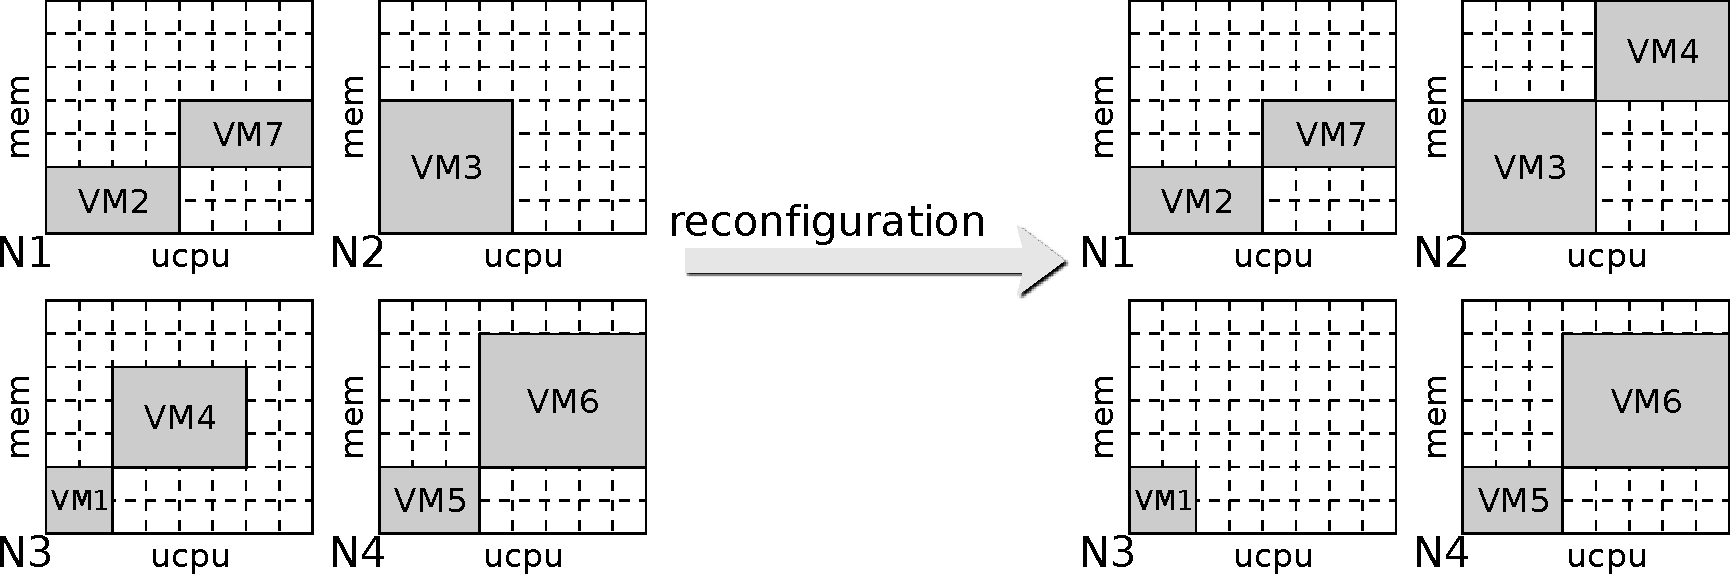
\includegraphics[width=\textwidth]{img/singleCapacity}
\caption{A reconfiguration motivated by \cstr{singleCapacity} constraints.}\label{fig: singleCapacity}
\end{figure}


\begin{itemize}
\item \cstr{singleCapacity(\{N1, N3\},4,"mem")}. This constraint was not satisfied in the source configuration
as the memory usage by the VMs on \cstr{N1} and \cstr{N3} equals 4 and 5, respectively.
This violation was fixed by relocating \cstr{VM4} to \cstr{N2} to liberate some resources.

\item \cstr{singleCapacity(\{N1, N2\},8,"ucpu")}. This constraint was satisfied in the source configuration
as the UCPU consumption of the running VMs was equals to 7 at maximum. The constraint is still satisfied
in the destination configuration as the relocation of \cstr{VM4} to \cstr{N2} makes the UCPU resource usage of \cstr{N2}
to 8, the maximum allowed.

\item \cstr{singleCapacity(\{N3\},1,"vm")}. This constraint was not satisfied in the source configuration
as the number of VMs running on \cstr{N3} was 2. The reconfiguration process fixed this violation by relocating
\cstr{VM4} to \cstr{N2}.
\end{itemize}

\fullVersion{
\subsection{Model}

\paragraph{Using the RP}

\subsection{Violation Detection}

The detection of the violating elements in \cstr{singleCapacity} consists in counting the VMs
that are hosted on each of the servers. When the amount of VMs exceed the maximum allowed, then
the difference indicates the minimum number of VMs that are misplaced. Such a detection is however
not capable to indicate the VMs that are actually misplaced.

\subsection{Availability}

\subsubsection{In BtrPlace}

Model depends on the content of \cstr{ns}. If it is a subset of the whole servers, then occurrence constraints. Otherwise, a bin packing constraint is preferable.
}

\subsection{See also}

\subsubsection{Related Constraints}
\begin{itemize}
\item \cstrref{cumulatedCapacity}: This constraint can be used when the resource restriction is related to the aggregation of some servers' resources.

\item \cstrref{preserve}: This constraint can be used in addition of \cstr{singleCapacity} constraint to ensure every VM has a sufficient amount of resources to run at peak level, according to the resources made available by \cstr{singleCapacity} constraints.

\end{itemize}

\emulatedWith{singleCapacity}{cumulatedCapacity}{\cstr{singleCapacity(ns, nb, r)}}{\cstr{\tforall n \tin ns, cumulatedCapacity(\{n\}, nb, r)}}
\printListOfInheritance{singleCapacity}